\documentclass[tikz,border=5pt]{standalone}
\usetikzlibrary{calc,intersections}
\tikzset{every node/.style={inner sep=0pt},every path/.style={thick,line cap=round,line join=round}}
\begin{document}
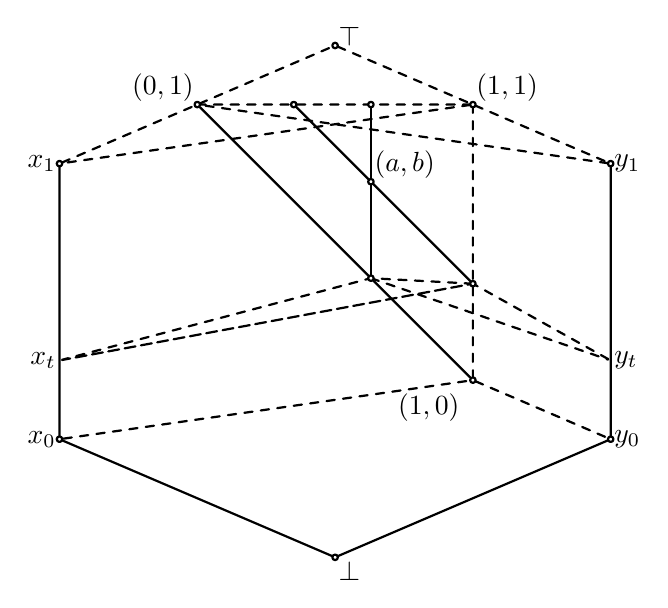
\begin{tikzpicture}[radius=1pt]
  \node[label=below right:$\perp$] (O1) {};
  \node[label=left:$x_0$] (x0) at (-3.5,1.5) {};
  \node[label=right:$y_0$] (y0) at (3.5,1.5) {};
  \node[label=left:$x_1$] (x1) at (-3.5,5) {};
  \node[label=right:$y_1$] (y1) at (3.5,5) {};
  \node[label={[yscale=-1]below right:$\perp$}] (O2) at (0,6.5) {};
  \node[label=left:$x_t$] (xt) at (-3.5,2.5) {};
  \node[label=right:$y_t$] (yt) at (3.5,2.5) {};
  \draw (x1) -- (x0)  -- (O1) -- (y0) -- (y1);
  \draw[dashed] (x1)  -- (O2) -- (y1);
  \draw[dashed] ($(O2)!.5!(y1)$) node[label=above right:{$(1,1)$}] (P1) {} -- ++(0,-3.5) node[label={[label distance=5pt]below left:{$(1,0)$}}] (P2) {} -- (x0) (P2) -- (y0) (P1) -- (x1);
  \draw[dashed] (y1) -- ($(O2)!.5!(x1)$) node[label=above left:{$(0,1)$}] (Q1) {} -- (P1);
  \draw ($(Q1)!.35!(P1)$) coordinate (Q4)  -- ($(P2)!.35!(P1)$) coordinate (Q2) (Q1) -- (P2);
  \draw[dashed] (Q2) -- ($(Q1)!.63!(P2)$) coordinate (Q3) -- (xt) -- (Q2) -- cycle (Q3) -- (yt) -- (Q2);
  \draw (Q3) -- ($(Q1)!.63!(P1)$) coordinate (Q5);
  \path[name path=line1] (Q4) -- (Q2);
  \path[name path=line2] (Q3) -- (Q5);
  \fill[white,draw=black,name intersections={of=line1 and line2}] (intersection-1) circle (1pt);
  \node[label=above right:{$(a,b)$}] at (intersection-1) {}; 
  \foreach \x in {O1,O2,x0,x1,y0,y1,Q1,Q2,Q3,Q4,Q5,P1,P2}
        \fill[white,draw=black] (\x) circle (1pt);
\end{tikzpicture}
\end{document}